\documentclass{standalone}
\usepackage{tikz}
\usetikzlibrary{intersections}

\tikzset{align at bottom/.style={baseline=(current bounding box.south)}}

\begin{document}
	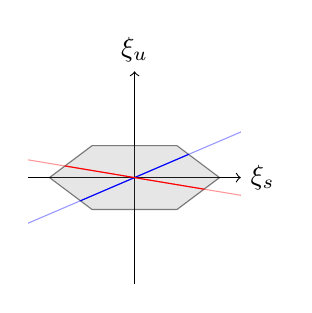
\begin{tikzpicture}[scale = 0.27]
	
		\draw[->] (-5, 0) -- (5, 0);
		\draw[->] (0, -5) -- (0, 5);
		\node[right] at (5, 0) {$\xi_s$};
		\node[above] at (0, 5) {$\xi_u$};
		
		\draw[draw = black, fill = gray, fill opacity = 0.2, draw opacity = 0.5, name path = support_cut_off] (-4, 0) -- (-2, 1.5) -- (2, 1.5) -- (4, 0) -- (2, -1.5) -- (-2, -1.5) -- cycle;
		
		\begin{scope}
			\clip (-5, -5) rectangle (5, 5);
			\draw[scale = 1, smooth, domain = -10 : 10, variable = \x, blue, opacity = 0.4, name path = plane1] plot ({\x},{ -1 / (- 7 / 3) * \x});
			\draw[scale=1, smooth, domain = -10 : 10, variable = \x, red, opacity = 0.4, name path = plane2] plot ({\x},{ -1 / (12 / 2) * \x});
			
			\draw[blue, name intersections = {of = support_cut_off and plane1}] (intersection-1) -- (intersection-2);
			\draw[red, name intersections = {of = support_cut_off and plane2}] (intersection-1) -- (intersection-2);
			
		\end{scope}
		
	\end{tikzpicture}
	
\end{document}